\documentclass[sigconf]{acmart}

\usepackage{hyperref}

%\usepackage{endfloat}
%\renewcommand{\efloatseparator}{\mbox{}} % no new page between figures

\usepackage{booktabs} % For formal tables

\settopmatter{printacmref=false} % Removes citation information below abstract
\renewcommand\footnotetextcopyrightpermission[1]{} % removes footnote with conference information in first column
\pagestyle{plain} % removes running headers


\begin{document}
\title{Big Data Analytics using Spark}


\author{Nisha Chandwani}
\orcid{1234-5678-9012}
\affiliation{%
  \institution{Indiana University Bloomington}
  \city{Bloomington} 
  \state{Indiana} 
  \postcode{47405}
}
\email{nchandwa@iu.edu}


% The default list of authors is too long for headers}
\renewcommand{\shortauthors}{B. Trovato et al.}


\begin{abstract}
With Petabytes of data being generated every second, big data analytics has become one of the most talked about terms in the technological world. Many organizations are trying to use big data for deriving useful business insights in order to improve decision making. However, we need special tools and frameworks to analyze such large amounts of data. We discuss how big data can be efficiently analyzed using Apache Spark which is a memory based computing framework. We discuss the core components and the architecture of Spark along with its ecosystem that extends the capabilities of Hadoop MapReduce. 

\end{abstract}

\keywords{i523, HID203, Apache Spark, RDD, Big Data Analytics, Hadoop, MapReduce}

\maketitle

\section{Introduction}

The growth of data has been following an exponential rate with huge amounts of data being generated every second. In today's world, having Terabytes or even Petabytes of data to deal with is not uncommon. The challenge lies not only in the volume of data but also in the large variance of the kind of data that has to be dealt with. This has led to the birth of one of the most talked about terms in today's technological world, i.e., Big Data. Most of the organizations today are collecting big data with the goal of extracting \emph{value} from the exploratory analysis of this data and using this information to make business decisions. However, analyzing such enormous data is in itself a huge challenge and this is where big data analytics frameworks like Spark come to rescue. Spark is a general distributed computing framework that is optimized for in-memory processing. We show how Spark supports faster data analysis and is proving to be one of the most successful frameworks for Big Data Analytics.


\section{Spark}

Spark is a general distributed computing framework which is based on Hadoop MapReduce algorithms\cite{fu2016spark-p1}. However, using Hadoop MapReduce for complex tasks requires frequent disk I/O which make Hadoop less suited for low-latency tasks. To overcome this, Spark extends the capability of MapReduce by providing in-memory computing which enables it to query data much faster than disk-based engines like Hadoop\cite{spark-j1}. Due to its memory computing capabilities, Spark is often used for iterative applications, such as Data Mining and Machine Learning\cite{fu2016spark-p1}. 

Apache Spark has a well-defined architecture which is based on two main abstractions\cite{spark-a2}:
\begin{itemize}
	\item Resilient Distributed Datasets (RDD)
	\item Directed Acyclic Graph (DAG)
\end{itemize}

\subsection{Resilient Distributed Datasets (RDD)} 
The entire framework of Spark is centered around RDD as it supports in-memory processing computation. This means it stores the state of memory in the form of an object across multiple jobs and the object is shared between these jobs\cite{spark-j2}. RDD is a collection of data items that can be operated in parallel and is stored in memory or on disk. This parallel data computing structure is read-only and is distributed over a cluster of machines offering a restricted form of distributed shared memory. RDDs are maintained in a fault-tolerant way and can cache intermediate data across a set of nodes. Thus, RDDs enable Spark to efficiently support iterative algorithms\cite{marcu2016spark-p2}.

RDD supports two types of operations\cite{spark-a3}:
\begin{itemize}
	\item Transformation: Operations like join, union, filter or map on existing RDDs which produce a new RDD as a result of the operation, are referred to as transformations.
	\item Action: Operations like count, first and reduce which evaluate an existing RDD and return values after computations are referred to as Actions.
\end{itemize}

\subsection{Directed Acyclic Graph (DAG)} 
Spark consists of an advanced Directed Acyclic Graph (DAG) engine which allows programmers to develop complex, multi-step data pipeline\cite{spark-a1}. Each Spark job creates a DAG of task stages to be executed on the cluster where each node in the DAG is an RDD partition and each edge represents a transformation to be applied on the data. This allows simple tasks to complete in a single stage whereas more complex tasks are completed in a single run of multiple stages, rather than splitting them into multiple jobs\cite{verma2016big-p3}. Thus, DAG abstraction eliminates the Hadoop MapReduce multi-stage execution model resulting in better performance\cite{spark-a2}.

\section{Spark Architecture and Hardware Introduction}
Spark is built in programming language Scala and is run on Java Virtual Machine (JVM). In addition to Scala, it provides API for Java and Python as well. For running an application, Spark provides the following two options\cite{verma2016big-p3}:
\begin{itemize}
	\item Interpreter in the Scala language distribution allows users to execute their queries on large data sets through Spark engine. 
	\item Users can write their applications as Scala programs called driver programs. These driver programs can be then compiled and submitted to the cluster's master node.
\end{itemize}

Apache Spark uses a master/worker architecture as shown in Figure 1. It mainly consists of a driver program (SparkContext), workers (executors) and a cluster manager which are described below\cite{spark-a2}: 

\begin{figure}
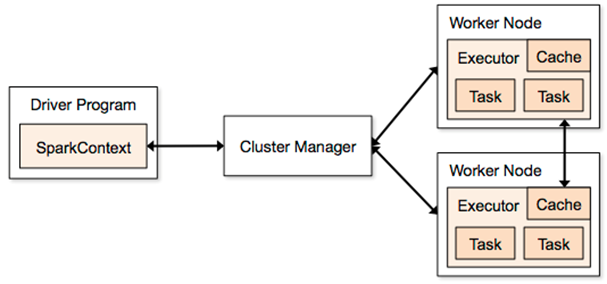
\includegraphics{images/spark-architecture}
\caption{Spark Architecture\cite{img-arch}}
\label{Figure 1}
\end{figure}

\begin{itemize}
	\item Driver Program: This program runs the main function of the Spark application. It is also responsible for the creation of the SparkContext object which basically coordinates the independent sets of processes running for an application on the cluster. The main components of the driver program are - DAGScheduler, TaskScheduler, BackendScheduler and BlockManager that translate the user code into Spark jobs that are executed on the cluster.
	\item Executor: These are the worker processes that are responsible for the execution of tasks sent by the SparkContext object. Some of these tasks include processing the data, reading from and writing data to external sources, performing computations and storing the results in in-memory cache or on hard disk drives.
	\item Cluster Manager: This is an external service that is responsible for acquiring resources on the Spark cluster and allocating them to the Spark jobs.
\end{itemize}

Being a memory-based computing platform, one of the most important factors of the Spark cluster is the memory. All the nodes, i.e., the driver and the executor nodes, should be equipped with at least 8 GB of memory for Spark to run well. For the cluster manager, Spark currently supports the below three deployments\cite{fu2016spark-p1}:

\begin{itemize}
	\item Standalone: It is a simple cluster manager included with Spark. Since Spark Standalone is available in the default configuration, it is the easiest way to set up a cluster and run applications on Spark.
	\item Apache Mesos: It is a general cluster manager that provides API for resource management and task scheduling across multiple nodes
	\item Hadoop YARN: It is the resource manager in Hadoop 2 which was added to Spark in version 0.6.
\end{itemize}

\section{Spark for Big Data Analytics}
With a large number of companies now looking to expand their advanced analytics capabilities, the ecosystem of Spark is right out of the box, making advanced analytics a reality. This ecosystem, as shown in Figure 2, provides an impressive set of high-level tools which include - Spark SQL for SQL, MLlib for machine learning, GraphX for graph processing and Spark Streaming\cite{fu2016spark-p1}. Each of these components is-

\begin{figure}
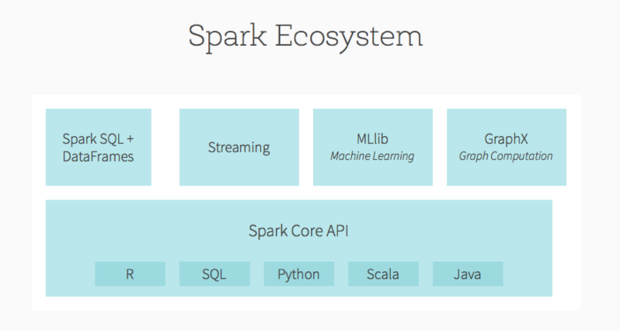
\includegraphics[height=3in, width=5in]{images/spark-ecosystem}
\caption{Spark Ecosystem\cite{img-echo}}
\label{Figure 2}
\end{figure}

\begin{itemize}

	\item Spark Core API is the foundation of the overall ecosystem that provides task scheduling, dispatching and basic I/O functionalities. It is available through API in languages like Java, Python, Scala and R.

  \item Spark SQL is Apache's Spark module for supporting SQL implementation. It provides seamless integration of SQL queries with Spark programs. It provides a common way to connect to a variety of data sources such as Hive, JSON, JDBC, etc.
  
  \item Spark Streaming is an extension to the core Spark API which provides the capability to process streaming jobs along with batch jobs. The languages supported are Java, Python and Scala.

  \item MLlib is Spark's scalable Machine Learning library which is usable in Java, Python, Scala and R. MLlib supports high-quality algorithms such as classification, regression, clustering, recommendation, dimensionality reduction, etc. MLlib leverages Spark's excellence in iterative computing enabling it to run faster than MapReduce on huge datasets.

  \item GraphX is Spark's parallel computation API used for charts and graphs processing\cite{fu2016spark-p1}. GraphX extends the capabilities of Spark RDD by introducing RDD graph which is a directed multi-graph with properties connected to each node and the edge\cite{spark-a1}. 
  
\end{itemize}

One of the challenges of analyzing big data is that it can come in any shape or size. Thus, whether big data is to be processed offline (Spark Core) or on the fly (Spark Streaming), whether it is structured (Spark SQL) or connected in nature (GraphX), Spark ecosystem is a framework that can be widely used in big data analytics.

\section{Spark versus Hadoop MapReduce}
Both Spark and Hadoop MapReduce are widely used in big data analytics, however, Spark has some major use cases over Hadoop\cite{verma2016big-p3}:
\begin{itemize}
	\item Unlike Hadoop, Spark supports interactive data mining and data processing
  \item Spark outperforms Hadoop when it comes to iterative algorithms in machine learning as it keeps working sets in memory for efficient reuse  
  \item Spark supports efficient stream processing which is one of the major advantages over Hadoop
  \item Spark is faster than MapReduce in execution
\end{itemize}

Though Spark has many advantages, Hadoop MapReduce can prove to be more efficient when it comes to batch processing for data with size greater than the available memory.

\section{Conclusion}
With the increasing volume of data, big data analytics is only going to become more critical for businesses decisions. Analyzing data at a huge scale presents many challenges and as we showed, Apache Spark can be very useful in overcoming these challenges. Over past few years, though Hadoop MapReduce has been one of the prime big data analytics framework, we showed how Spark has some major use cases over Hadoop. Though Apache Spark is a relatively young data project, it has already been adopted by a wide range of industries for big data analytics. We provided an introduction to Spark and discussed its architecture and the core components. As future work, we can discuss a case study and show how Spark processes big data in a more efficient manner than Hadoop MapReduce.

\begin{acks}

  We would like to thank Prof. Gregor von Laszewski and the teaching assistants for their helpful suggestions. 

\end{acks}

\bibliographystyle{ACM-Reference-Format}
\bibliography{report} 

\section{Bibtex Issues}
\todo[inline]{Warning--empty year in img-arch}
\todo[inline]{Warning--no journal in spark-a3}
\todo[inline]{Warning--no number and no volume in spark-a3}
\todo[inline]{Warning--page numbers missing in both pages and numpages fields in spark-a3}
\todo[inline]{Warning--no journal in spark-a2}
\todo[inline]{Warning--no number and no volume in spark-a2}
\todo[inline]{Warning--page numbers missing in both pages and numpages fields in spark-a2}
\todo[inline]{Warning--empty publisher in fu2016spark-p1}
\todo[inline]{Warning--empty address in fu2016spark-p1}
\todo[inline]{Warning--empty year in spark-j2}
\todo[inline]{Warning--no journal in spark-j2}
\todo[inline]{Warning--no number and no volume in spark-j2}
\todo[inline]{Warning--page numbers missing in both pages and numpages fields in spark-j2}
\todo[inline]{Warning--empty publisher in marcu2016spark-p2}
\todo[inline]{Warning--empty address in marcu2016spark-p2}
\todo[inline]{Warning--no journal in spark-a1}
\todo[inline]{Warning--no number and no volume in spark-a1}
\todo[inline]{Warning--page numbers missing in both pages and numpages fields in spark-a1}
\todo[inline]{Warning--page numbers missing in both pages and numpages fields in spark-j1}
\todo[inline]{Warning--empty publisher in verma2016big-p3}
\todo[inline]{Warning--empty address in verma2016big-p3}
\todo[inline]{(There were 21 warnings)}
\section{Issues}

\DONE{Example of done item: Once you fix an item, change TODO to DONE}

\subsection{Assignment Submission Issues}

    \TODO{Do not make changes to your paper during grading, when your repository should be frozen.}

\subsection{Uncaught Bibliography Errors}

    \TODO{Missing bibliography file generated by JabRef}
    \TODO{Bibtex labels cannot have any spaces, \_ or \& in it}
    \TODO{Citations in text showing as [?]: this means either your report.bib is not up-to-date or there is a spelling error in the label of the item you want to cite, either in report.bib or in report.tex}

\subsection{Formatting}

    \TODO{Incorrect number of keywords or HID and i523 not included in the keywords}
    \TODO{Other formatting issues}

\subsection{Writing Errors}

    \TODO{Errors in title, e.g. capitalization}
    \TODO{Spelling errors}
    \TODO{Are you using {\em a} and {\em the} properly?}
    \TODO{Do not use phrases such as {\em shown in the Figure below}. Instead, use {\em as shown in Figure 3}, when referring to the 3rd figure}
    \TODO{Do not use the word {\em I} instead use {\em we} even if you are the sole author}
    \TODO{Do not use the phrase {\em In this paper/report we show} instead use {\em We show}. It is not important if this is a paper or a report and does not need to be mentioned}
    \TODO{If you want to say {\em and} do not use {\em \&} but use the word {\em and}}
    \TODO{Use a space after . , : }
    \TODO{When using a section command, the section title is not written in all-caps as format does this for you}\begin{verbatim}\section{Introduction} and NOT \section{INTRODUCTION} \end{verbatim}

\subsection{Citation Issues and Plagiarism}

    \TODO{It is your responsibility to make sure no plagiarism occurs. The instructions and resources were given in the class}
    \TODO{Claims made without citations provided}
    \TODO{Need to paraphrase long quotations (whole sentences or longer)}
    \TODO{Need to quote directly cited material}

\subsection{Character Errors}

    \TODO{Erroneous use of quotation marks, i.e. use ``quotes'' , instead of " "}
    \TODO{To emphasize a word, use {\em emphasize} and not ``quote''}
    \TODO{When using the characters \& \# \% \_  put a backslash before them so that they show up correctly}
    \TODO{Pasting and copying from the Web often results in non-ASCII characters to be used in your text, please remove them and replace accordingly. This is the case for quotes, dashes and all the other special characters.}
    \TODO{If you see a figure and not a figure in text you copied from a text that has the fi combined as a single character}

\subsection{Structural Issues}

    \TODO{Acknowledgement section missing}
    \TODO{Incorrect README file}
    \TODO{In case of a class and if you do a multi-author paper, you need to add an appendix describing who did what in the paper}
    \TODO{The paper has less than 2 pages of text, i.e. excluding images, tables and figures}
    \TODO{The paper has more than 6 pages of text, i.e. excluding images, tables and figures}
    \TODO{Do not artificially inflate your paper if you are below the page limit}

\subsection{Details about the Figures and Tables}

    \TODO{Capitalization errors in referring to captions, e.g. Figure 1, Table 2}
    \TODO{Do use {\em label} and {\em ref} to automatically create figure numbers}
    \TODO{Wrong placement of figure caption. They should be on the bottom of the figure}
    \TODO{Wrong placement of table caption. They should be on the top of the table}
    \TODO{Images submitted incorrectly. They should be in native format, e.g. .graffle, .pptx, .png, .jpg}
    \TODO{Do not submit eps images. Instead, convert them to PDF}

    \TODO{The image files must be in a single directory named "images"}
    \TODO{In case there is a powerpoint in the submission, the image must be exported as PDF}
    \TODO{Make the figures large enough so we can read the details. If needed make the figure over two columns}
    \TODO{Do not worry about the figure placement if they are at a different location than you think. Figures are allowed to float. For this class, you should place all figures at the end of the report.}
    \TODO{In case you copied a figure from another paper you need to ask for copyright permission. In case of a class paper, you must include a reference to the original in the caption}
    \TODO{Remove any figure that is not referred to explicitly in the text (As shown in Figure ..)}
    \TODO{Do not use textwidth as a parameter for includegraphics}
    \TODO{Figures should be reasonably sized and often you just need to
  add columnwidth} e.g. \begin{verbatim}/includegraphics[width=\columnwidth]{images/myimage.pdf}\end{verbatim}

re\end{document}
